\documentclass[a4paper,12pt]{article}
\usepackage{xcolor}
\usepackage{amsmath,amsfonts,amssymb}
\usepackage{geometry}
\usepackage{fancyhdr}
\usepackage{graphicx}
\usepackage{titlesec}
\usepackage{tikz}
\usepackage{booktabs}
\usepackage{array}
\usetikzlibrary{shadows}
\usepackage{tcolorbox}
\usepackage{float}
\usepackage{lipsum}
\usepackage{mdframed}
\usepackage{pagecolor}
\usepackage{mathpazo}   % Palatino font (serif)
\usepackage{microtype}  % Better typography
\usepackage{url}

\setlength{\parindent}{0pt}

% Page background color
\pagecolor{gray!10!white}

% Geometry settings
\geometry{margin=0.5in}
\pagestyle{fancy}
\fancyhf{}

% Fancy header and footer
\fancyhead[C]{\textbf{\color{blue!80}The Diamond Shield}}
% \fancyhead[R]{\color{blue!80}Saksham Rathi}
\fancyfoot[C]{\thepage}

% Custom Section Color and Format with Sans-serif font
\titleformat{\section}
{\sffamily\color{purple!90!black}\normalfont\Large\bfseries}
{\thesection}{1em}{}

% Custom subsection format
\titleformat{\subsection}
{\sffamily\color{cyan!80!black}\normalfont\large\bfseries}
{\thesubsection}{1em}{}

% Stylish Title with TikZ (Enhanced with gradient)
\newcommand{\cooltitle}[1]{%
\begin{tikzpicture}
\node[fill=blue!20,rounded corners=10pt,inner sep=12pt, drop shadow, top color=blue!50, bottom color=blue!30] (box)
{\Huge \bfseries \color{black} #1};
\end{tikzpicture}
}
\usepackage{float} % Add this package

\newenvironment{solution}[2][]{%
\begin{mdframed}[linecolor=blue!70!black, linewidth=2pt, roundcorner=10pt, backgroundcolor=yellow!10!white, skipabove=12pt, skipbelow=12pt]%
	\textbf{\large #2}
	\par\noindent\rule{\textwidth}{0.4pt}
}{
\end{mdframed}
}

% Document title
\title{\cooltitle{CS790 Assignment 1} \\
\LARGE \textbf{The Diamond Shield} \\
Report}
\author{{\bf Kavya Gupta (22B1053)} \\
\small Department of Computer Science, \\
Indian Institute of Technology Bombay \\}
\date{}

\begin{document}
\maketitle

\section*{Task 1}

\begin{solution}{Setup}
    \begin{itemize}
        \item Used Oracle VirtualBox
        \item All 3 VMs are FreeBSD 13.4
        \item VM1 and 3 were assigned 1024MB RAM and 1 CPU and VM2 was assigned 2048MB RAM and 2 CPUs
    \end{itemize}
\end{solution}

\begin{solution}{Part (a): Configuring the Network}
    The steps followed are:-
    \begin{enumerate}
        \item In the ``Network'' section of the VM settings, I added a new ``Internal Network'' for each VM for the inter-VM communication.\ \texttt{intnet} for VM2-3 and \texttt{intnet2} for VM1-2.
        \begin{figure}[H]
            \centering
            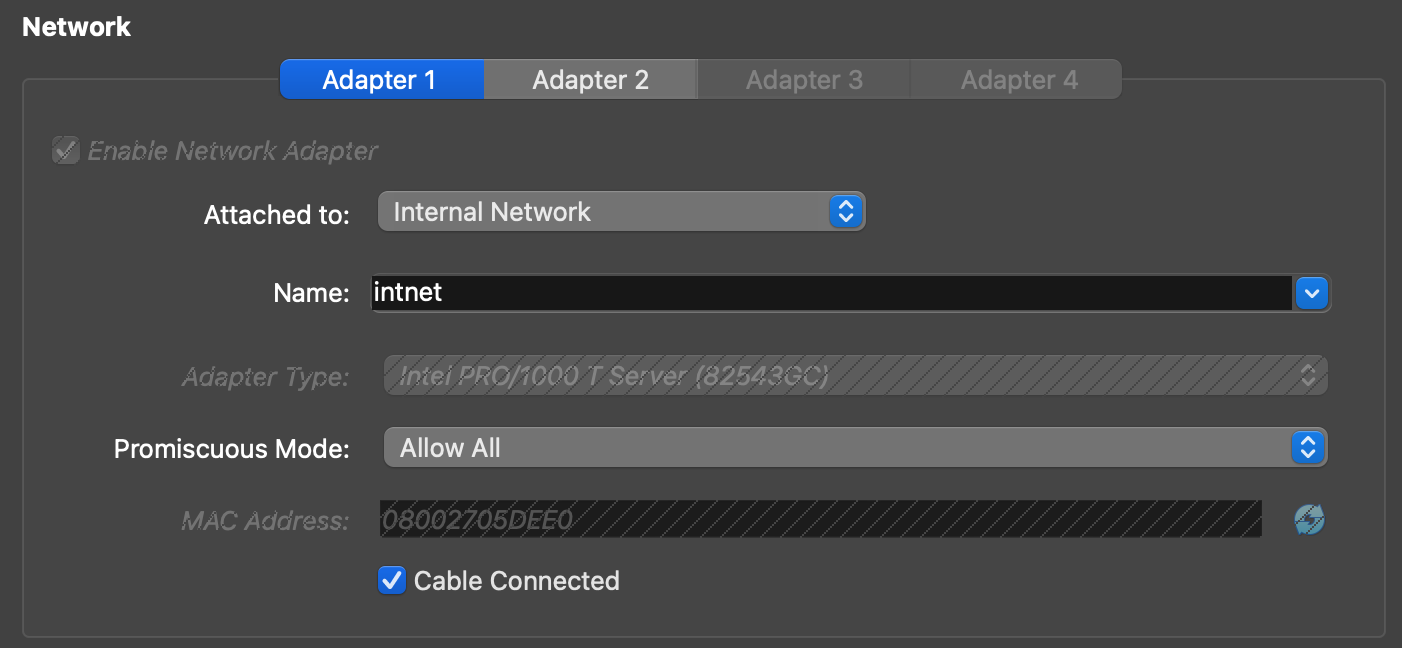
\includegraphics[width=0.4\textwidth]{internal_network.png}
        \end{figure}
        \item Inside the VM, I changed the name of interfaces (E.g.\ \texttt{em0} to \texttt{eth0} in VM1 and 3) and assigned static IP addresses to the interfaces.\ To achieve this, I added the following lines to the \texttt{/etc/rc.conf} file (these are for VM1, similar for VM2 and 3):-
        \begin{itemize}
            \item \texttt{ifconfig\_em0\_name="eth0"}
            \item \texttt{ifconfig\_eth0="inet 192.168.10.2 netmask 255.255.255.0 up"}
        \end{itemize}
        These are the IP addresses assigned to the interfaces:-
        \begin{itemize}
            \item VM1 \texttt{eth0}: \texttt{192.168.10.2}
            \item VM2 \texttt{eth0}: \texttt{192.168.10.1}, \texttt{eth1}: \texttt{192.168.20.1}
            \item VM3 \texttt{eth0}: \texttt{192.168.20.2}
        \end{itemize}
        Hence VM1 and 2 belong to the \texttt{192.168.10.0/24} subnet and VM2 and 3 belong to the \texttt{192.168.20.0/24} subnet.
    \end{enumerate}
\end{solution}

\begin{solution}{Part (b): Enabling IP Forwarding}
    The steps followed are:-
    \begin{enumerate}
        \item Added \texttt{gateway\_enable="YES"} to the \texttt{/etc/rc.conf} file of VM2.
        \item Added \texttt{net.inet.ip.forwarding=1} to the \texttt{/etc/sysctl.conf} file of VM2.
        \item Made a new static route (to VM3) in VM1 by adding the following line to the \texttt{/etc/rc.conf} file of VM1:-
        \begin{itemize}
            \item \texttt{static\_routes="net20"}
            \item \texttt{route\_net20="-net 192.168.20.0/24 192.168.10.1"}
        \end{itemize}
        \item Similarly made a new static route (to VM1) in VM3.
    \end{enumerate}
    Note: Routing table can be checked using the \texttt{netstat -r} command.

    Traceroute from VM1 to VM3 shows that it goes via VM2:-
    \begin{figure}[H]
        \centering
        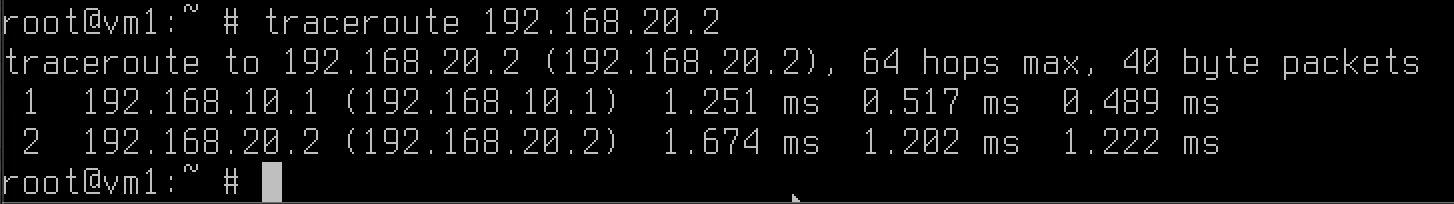
\includegraphics[width=0.6\textwidth]{traceroute.png}
    \end{figure}
\end{solution}

\begin{solution}{Part (c): Communicating using HTTP}
    The steps followed are:-
    \begin{enumerate}
        \item To enable Internet access in VM3, I added a ``Bridged Adapter'' to VM3's ``Network'' section.\ Also had to run \texttt{dhclient em1} to get an IP address.
        \item Installed the Apache web server in VM3 using the command \texttt{pkg install apache24}.
        \item Started the Apache service using the command \texttt{service apache24 start}.\ Also added \texttt{apache24\_enable="YES"} to the \texttt{/etc/rc.conf} file.
        \item Ensured that \texttt{LISTEN 80} is there in the \texttt{/usr/local/etc/apache24/httpd.conf} file.\ Also had to change the \texttt{ServerName} to \texttt{192.168.20.2:80}.
        \item Files to be shared are supposed to be in the \texttt{/usr/local/www/apache24/data} directory.\ By default, the \texttt{index.html} file is there.
        \item Installed the \texttt{wget} package in VM1 using the command \texttt{pkg install wget}.\ Then ran the command \texttt{wget http://192.168.20.2/index.html}, the results are shown below:-
        \begin{figure}[H]
            \centering
            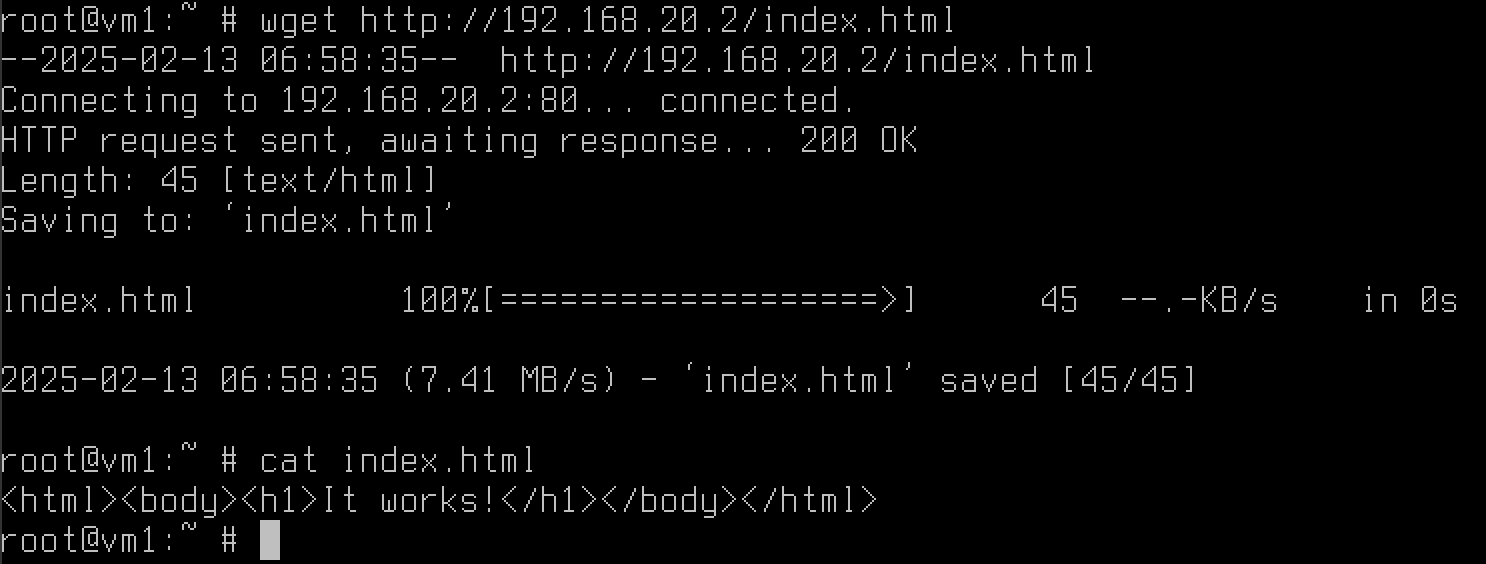
\includegraphics[width=0.6\textwidth]{wget.png}
        \end{figure}
    \end{enumerate}
\end{solution}

\begin{solution}{Part (d): Packet Filtering using \texttt{pf}}
    The steps followed are:-
    \begin{enumerate}
        \item Added the following lines to the \texttt{/etc/pf.conf} file of VM2:-
        \begin{itemize}
            \item \texttt{block in on eth0 inet from 192.168.10.2 to 192.168.20.2}
            \item \texttt{block out on eth1 inet from 192.168.10.2 to 192.168.20.2}
            \item \texttt{pass in on eth0 inet proto tcp from 192.168.10.2 to 192.168.20.2 port 80}

            \texttt{keep state}
            \item \texttt{pass out on eth1 inet proto tcp from 192.168.10.2 to 192.168.20.2 port}

            \texttt{80 keep state}
        \end{itemize}
        The first two lines make sure that any traffic from VM1 to VM3 via VM2 is blocked.\ The next two lines allow ONLY the HTTP traffic through this route.
        \item Enabled the \texttt{pf} service using the command \texttt{pfctl -e}.\ Also added \texttt{pf\_enable="YES"} to the \texttt{/etc/rc.conf} file of VM2.
        \item Uploaded the rules using the command \texttt{pfctl -f /etc/pf.conf}.
        
        Note: \texttt{pf} can be disabled using the command \texttt{pfctl -d}.
    \end{enumerate}
    Below is the output of \texttt{ssh} from VM1 to VM3 with \texttt{pf} disabled:-
    \begin{figure}[H]
        \centering
        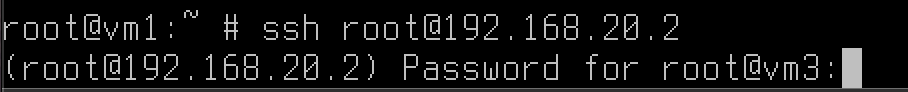
\includegraphics[width=0.6\textwidth]{ssh_with_no_pf.png}
    \end{figure}
    And below is the same but with \texttt{pf} enabled:-
    \begin{figure}[H]
        \centering
        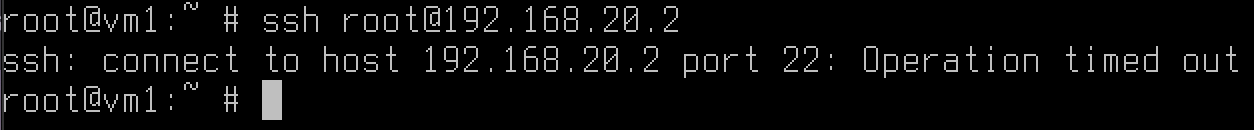
\includegraphics[width=0.6\textwidth]{ssh_with_pf.png}
    \end{figure}
    Now, the output of \texttt{wget} from VM1 to VM3 with \texttt{pf} enabled is as in the figure of previous part.

\end{solution}

\begin{solution}{References}
    \begin{itemize}
        \item FreeBSD Handbook, Docs.\ VirtualBox Manual.\ The book of pf.
        \item \url{https://www.nakivo.com/blog/virtualbox-network-setting-guide/}
    \end{itemize}
\end{solution}

\newpage

\section*{Task 2}

\begin{solution}{Files Submitted}
    \begin{itemize}
        \item \texttt{icmp\_block.c}
        \item \texttt{Makefile}
    \end{itemize}
\end{solution}

\begin{solution}{Instructions to Execute the Code}
    Make sure that \texttt{Makefile} and \texttt{icmp\_block.c} are present in the same directory. In that directory:-
    \begin{enumerate}
        \item Run \texttt{make} to compile the kernel module.
        \item Run \texttt{pfctl -d} to ensure that \texttt{pf} is disabled.
        \item Run \texttt{kldload ./icmp\_block.ko} to load the kernel module.
        \item Run \texttt{kldunload icmp\_block} to unload the module.
    \end{enumerate}
    Note: All of this was done as the root user.
\end{solution}

\begin{solution}{Little Overview of the Code}
    \begin{itemize}
        \item \texttt{icmp\_block\_hook}: This is the hook function that is ran over each IP packet and blocks those with the ICMP Protocol and Echo Request type and inward direction.\ \texttt{PFIL\_IN} is used for it.
        \item \texttt{load\_handler}: This function is called when the module is loaded/unloaded. It adds \texttt{icmp\_block\_hook} to the hooks list and links it with the \texttt{inet} head in inward direction.
    \end{itemize}
\end{solution}

\begin{solution}{Additional Steps}
    \begin{itemize}
        \item Ran \texttt{wget https://download.freebsd.org/releases/arm64/13.4-RELEASE/src.txz} and un-tared it at \texttt{/usr/src} to get the kernel source modules.
        \item Installed \texttt{gcc} and \texttt{make} using the command \texttt{pkg install gcc gmake}.
        \item Used {\small \url{https://tylersguides.com/guides/how-to-increase-the-size-of-a-freebsd-disk/}}
        
        to increase the disk size of VM2.
        \item \texttt{pfilctl heads} and \texttt{pfilctl hooks} give us currently active heads and hooks respectively.
    \end{itemize}
\end{solution}

\begin{solution}{Output}
    This is the output of \texttt{pfilctl heads} after loading the module:-
    \begin{figure}[H]
        \centering
        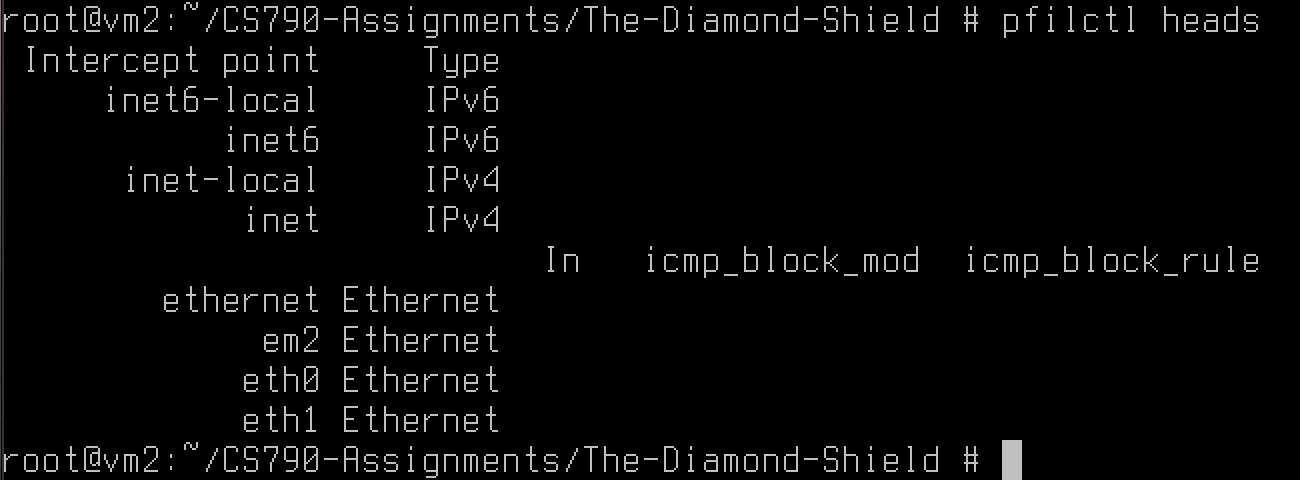
\includegraphics[width=0.6\textwidth]{pfilctl.png}
    \end{figure}
    This is the output of \texttt{ping} from VM1 to VM3 with the module loaded:-
    \begin{figure}[H]
        \centering
        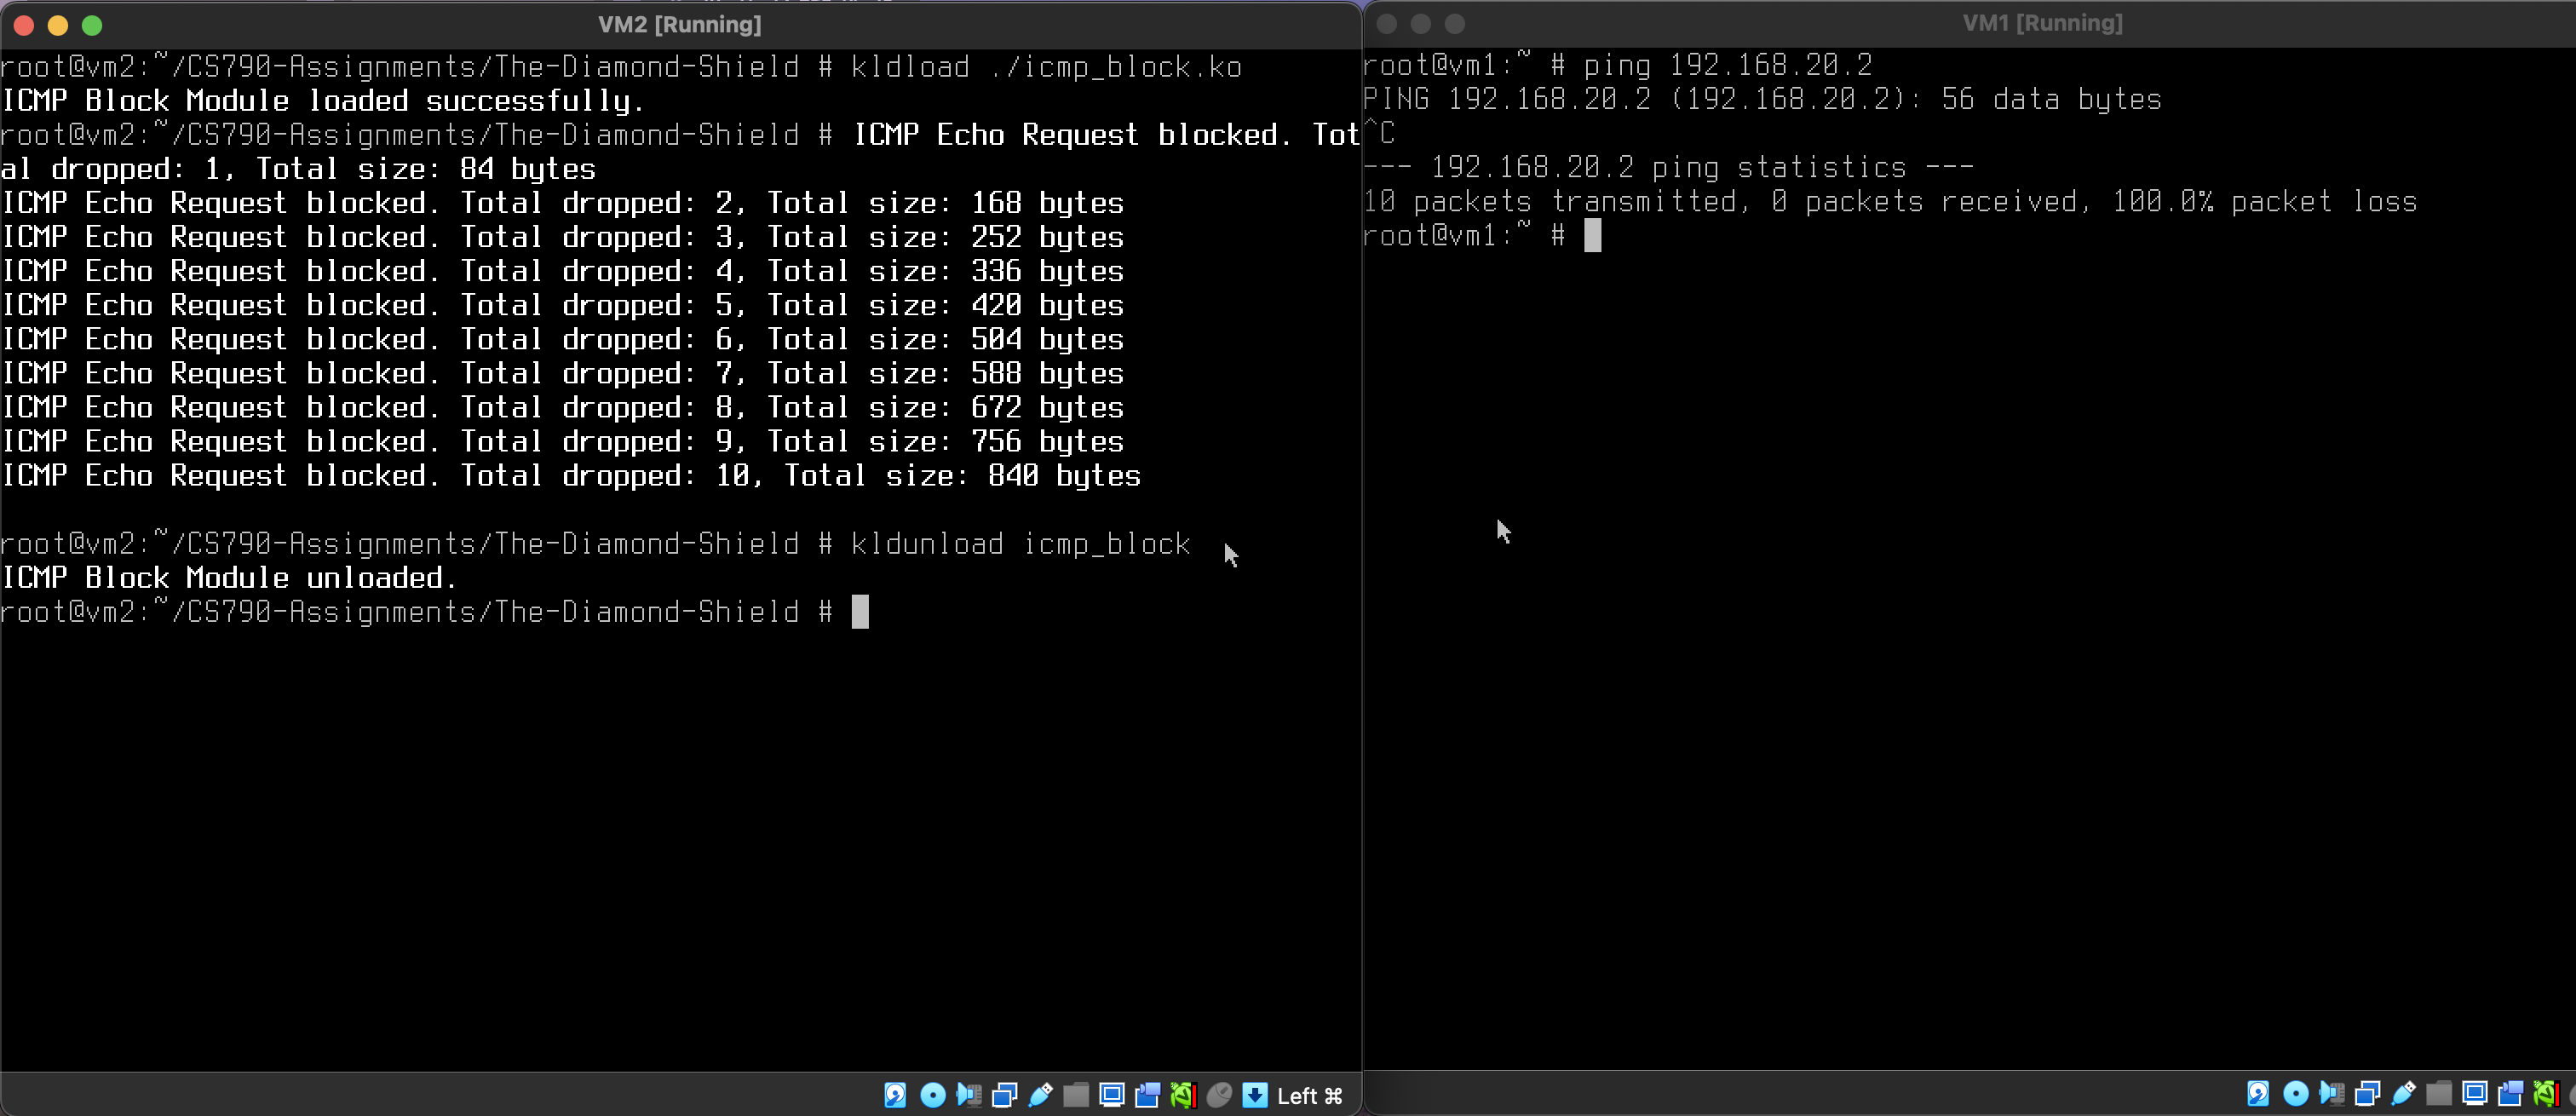
\includegraphics[width=0.6\textwidth]{task-2.png}
    \end{figure}
    As you can see that the packets are successfully being dropped.
\end{solution}

\begin{solution}{Resources Used}
    \begin{itemize}
        \item Used a little bit of ChatGPT to get a headstart.\ Got the idea to use the \texttt{net/pfil.h} library.
        \item Used the man pages of \texttt{pfil(9)} to get idea of the functions to be used.
        \item At \url{http://fxr.watson.org/fxr/source/net/pfil.h?v=FREEBSD-13-0}, found the source code of \texttt{pfil.h} (and of \texttt{pfil.c} similarly).
        \item {\small \url{https://medium.com/rossdotpink/writing-a-simple-freebsd-kernel-module-9302bd4cfae1}}
    \end{itemize}
\end{solution}

\end{document}